\documentclass[10pt]{article}
\usepackage[margin=0.8in]{geometry}
\usepackage{booktabs,longtable,graphicx,hyperref}
\title{Experiment03B: Frame-Ranking Validation and Integrity Amendment R1}
\author{Research report for Shrid Pant}\date{October 26, 2026}
\begin{document}\maketitle
\begin{abstract}
Across the original VERA alert population, blur-ranked frame pairs removed alerts under grey replacement more often than the exhaustive pair reference. The original result is preserved. A separately versioned, post-data integrity audit resolves four validator-contract defects without rerunning inference or altering any original score, label, rank or result. This establishes the declared perturbation effect, not semantic faithfulness or improved detection.
\end{abstract}
\section{Design and coverage}
The frozen InternVL2-8B model answers the original VERA explanation-first prompt on eight sampled frames per window. A separate label-only scorer ranks frames by singleton blur effects. Evaluation replaces the top two with grey and compares the original VERA alert flip with the exact mean over all 28 pairs. Blur and grey are distribution-shifting interventions, not natural missingness.

The manifest covers 290 UCF-Crime test videos, 452 window records and 433 unique available inputs. Nineteen negative-window records are unavailable. Excluding the two development videos leaves 430 inputs from 288 video IDs. The primary population contains 199 alerts across 138 videos, with no missing primary effects. Event-centred windows use benchmark interval information and are oracle-localized. This is not a benchmark-wide detection evaluation.
\section{Primary result}
The original video-weighted advantage is \textbf{15.166 percentage points}, 95\% interval $[9.860,20.600]$. The video-cluster bootstrap uses 10,000 draws and seed 0. Bootstrap stability seeds are numerical checks, not independent experiments.
\begin{figure}[ht]\centering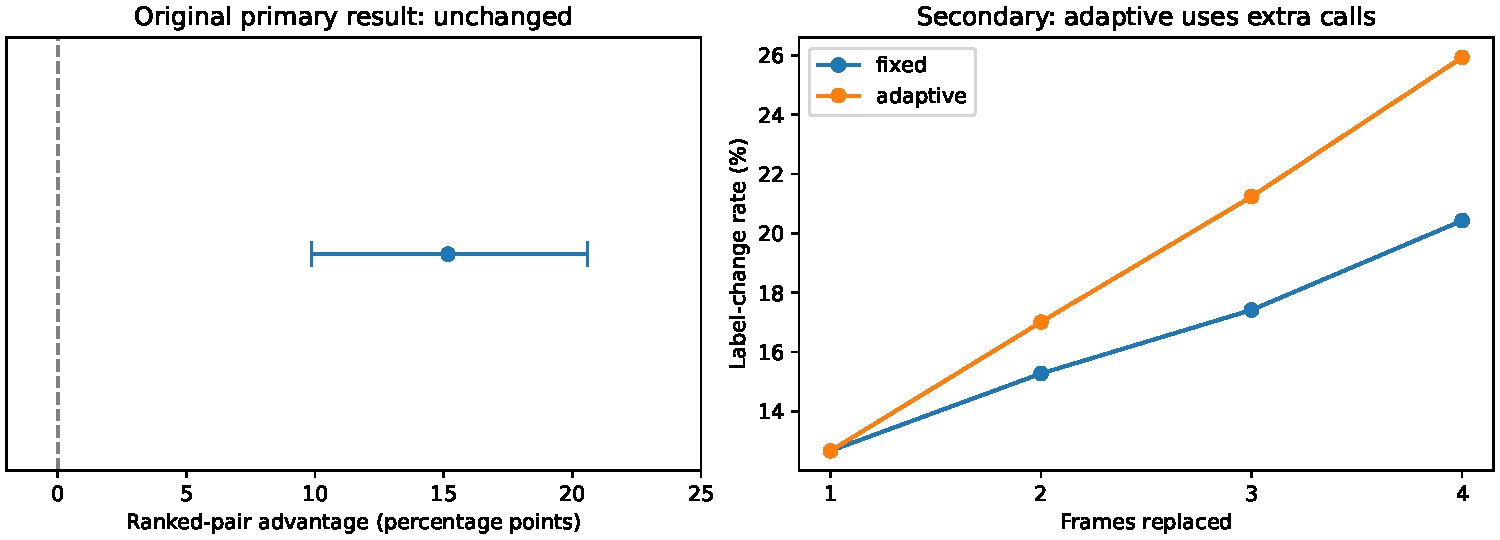
\includegraphics[width=\linewidth]{results.pdf}\caption{Original primary result and secondary prefix behavior. Adaptive ranking costs more queries; this is not an equal-compute comparison.}\end{figure}
\section{Prespecified descriptive table}
\small\begin{longtable}{p{5.3cm}rrrrrr}\toprule Population & Videos & Windows & Alerts & Top-2 (\%) & Random (\%) & Gain (pp)\\\midrule\endhead
All original alerts, confirmation set & 288 & 430 & 199 & 26.8 & 11.6 & 15.2 \\
Event-centered windows & 139 & 161 & 126 & 18.0 & 7.7 & 10.3 \\
Annotation-free anomaly-video windows & 120 & 120 & 56 & 33.9 & 14.7 & 19.3 \\
Normal-video windows & 149 & 149 & 17 & 52.9 & 24.2 & 28.8 \\
Abuse & 2 & 4 & 2 & 50.0 & 39.3 & 10.7 \\
Arrest & 5 & 10 & 6 & 10.0 & 2.5 & 7.5 \\
Arson & 9 & 18 & 11 & 16.7 & 5.7 & 11.0 \\
Assault & 3 & 7 & 4 & 0.0 & 6.0 & -6.0 \\
Burglary & 13 & 27 & 17 & 25.0 & 8.3 & 16.7 \\
Explosion & 21 & 42 & 29 & 22.2 & 9.9 & 12.3 \\
Fighting & 5 & 10 & 8 & 30.0 & 6.8 & 23.2 \\
RoadAccidents & 22 & 36 & 22 & 23.3 & 7.0 & 16.3 \\
Robbery & 5 & 9 & 6 & 20.0 & 7.9 & 12.1 \\
Shooting & 23 & 48 & 34 & 26.2 & 8.4 & 17.8 \\
Shoplifting & 21 & 45 & 27 & 26.3 & 13.1 & 13.3 \\
Stealing & 5 & 12 & 6 & 20.0 & 31.4 & -11.4 \\
Vandalism & 5 & 13 & 10 & 20.0 & 3.1 & 16.9 \\
Sensitivity: including development videos & 290 & 433 & 200 & 27.3 & 11.9 & 15.4 \\
\bottomrule\end{longtable}\normalsize
Category and stratum rows are descriptive, not separate confirmatory tests. Gains refer to alert removal, not accuracy improvements.
\section{Integrity amendment: original 16/20, R1 20/20}
The original validator and its failed artifact remain unchanged. R1 reruns the original validator and replaces only four checks with explicitly documented contracts; the other sixteen pass unchanged. All 36 local source-run files (31 portable record files) are SHA256-identical before and after the audit.
\begin{enumerate}
\item \textbf{Numerical readouts.} The old validator demanded exact BF16 round-to-nearest, while the inference engine's existing contract used half a BF16 step plus $10^{-3}$ slack. R1 requires finite, representable BF16 values, verifies that pre-existing bound and the exact stored score difference, and retains every exact-rounding mismatch. This does not claim exact rounding or change rankings.
\item \textbf{Slot-hash flags.} The legacy flag means exactly the masked slots changed. R1 verifies that flag against recorded baseline tensors, rather than requiring it always be true.
\item \textbf{No-op blur.} Two hash-verified source frames are all black. Resizing and applying Gaussian blur with radius 17.92 leaves their pixels unchanged. Twenty records therefore contain valid no-op replacements. R1 permits only source-verified black-frame blur no-ops; unchanged grey replacements or unexplained unchanged masks fail. Unmasked slots must remain identical and repeated replacements must have consistent hashes.
\item \textbf{Cache aliases.} Different video names may identify identical content. Shared keys are allowed only when source hash, frame indices, frame hashes, family, mask and tensor hashes agree. Archived Normal Videos 936 and 937 independently hash to the same SHA256. Eighty-eight shared sequence keys are explained this way; distinct content sharing a key still fails.
\end{enumerate}
There are 45 exact-rounding mismatch records; the largest excess beyond half a step is 0.000171661, below the historical 0.001 slack.
\section{Duplicate-source sensitivity (post-data)}
The original analysis is retained. The sensitivity groups by source SHA256 and averages within source before averaging across sources. The duplicate pair is absent from the primary alert population: the primary point estimate is unchanged. Secondary population size falls from 288 IDs to 287 sources (430 rows contain 429 distinct window contents).
\begin{center}\begin{tabular}{lrrr}\toprule Metric & Original & Source-deduplicated & Sources\\\midrule
Primary advantage (pp) & 15.1656 & 15.1656 & 138 \\
Numeric margin (nats) & 0.3556 & 0.3559 & 287 \\
Blur/grey top-two overlap & 1.3935 & 1.3914 & 287 \\
No-sound changes (\%) & 5.2662 & 5.2846 & 287 \\
\bottomrule\end{tabular}\end{center}
All stored sensitivity metrics and prefix rates are in duplicate\_sensitivity.json. These are disclosed post-data checks, not replacements for the prespecified estimate.
\begin{figure}[ht]\centering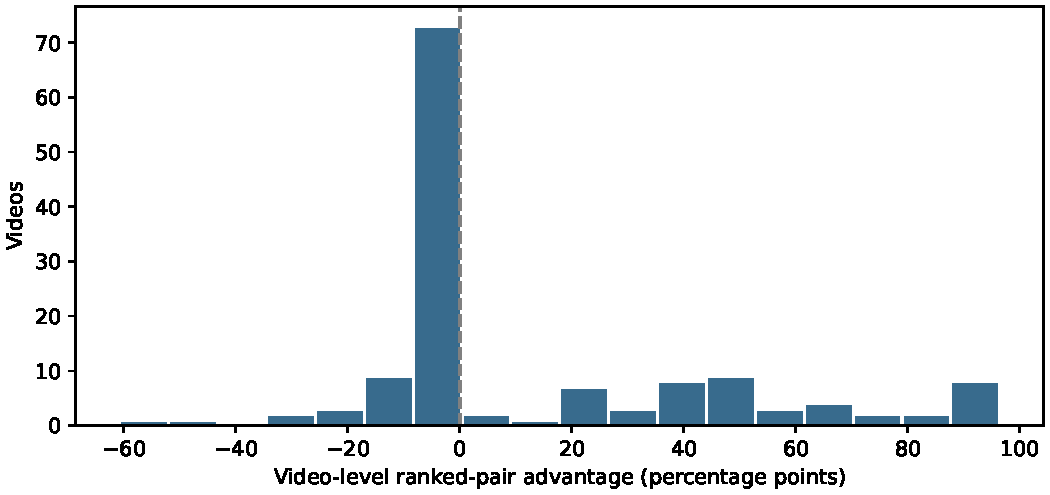
\includegraphics[width=.8\linewidth]{heterogeneity.pdf}\caption{Heterogeneity across the 138 primary video-level effects. A positive average does not imply each video's ranking is informative.}\end{figure}
\section{Scientific interpretation and limitations}
The result supports ranking utility for this local perturbation task. It does not establish that textual explanations identify human-valid evidence. The scorer and original VERA use different prompts; agreement must be measured. False alerts can also be fragile under deletion. The no-sound diagnostic changes labels but does not itself prove improvement. Heatmaps from prior feasibility work are not validated explanations. Source duplication is only one form of dependence; a source-hash audit cannot detect all related scenes or near-duplicate recordings.

This study targets local eight-frame judgments, not the ImageBind-refined timeline. Existing UCF test results have informed research decisions; future question learning needs disjoint development material and honest disclosure of evaluation reuse. No new question-learning experiment was launched.
\section{Reproduction and review}
The original frozen run is runs/full\_v1. The additive audit is audits/full\_v1\_r1; no model or GPU is needed. Run code/audit3b\_r1.py with the source run, a fresh audit directory, the original sparse frames, and experiment02 run\_002 for the precision-erratum check. Then run code/report3b\_r1.py against that audit. Exact commands, software versions, tests, hashes and amendment rationale are recorded in R1\_AMENDMENT.md and the audit JSON. Dataset images remain outside Git.\par
Review: \url{https://github.com/shridpant/VERA/pull/5}. The next experiment remains a decision for the researcher after reviewing this result.
\end{document}
